%% ============================================================
%% ESIT-D2I 2026 — Task 2: Machine Unlearning
%% Two unlearning families + a small ensemble
%% ============================================================
\documentclass[10pt]{beamer}
\usetheme[progressbar=frametitle,block=fill]{metropolis}
\metroset{sectionpage=none}   % lean talk: no section-divider slides

%% ---- packages -------------------------------------------------------
\usepackage{amsmath,amssymb,mathtools}
\usepackage{booktabs}
\usepackage{graphicx}
\usepackage{tikz}
\usetikzlibrary{shapes.geometric, arrows.meta, positioning, fit, backgrounds, calc}
\usepackage{xcolor}
\usepackage{array}
\usepackage{microtype}
\usepackage{appendixnumberbeamer}

%% ---- colors ---------------------------------------------------------
\definecolor{cForget}{RGB}{224,82,82}
\definecolor{cRetain}{RGB}{74,144,217}
\definecolor{cTeacher}{RGB}{170,170,170}
\definecolor{cAccent}{RGB}{243,166,18}

%% ---- macros ---------------------------------------------------------
\newcommand{\Rset}{\mathcal{R}}           % retain set
\newcommand{\Fset}{\mathcal{F}}           % forget set
\newcommand{\fth}{f_{\theta}}             % student model
\newcommand{\fthn}{f_{\theta_0}}          % frozen teacher
\newcommand{\yi}{\mathbf{y}_i}            % original label
\newcommand{\ycorr}{\hat{\mathbf{y}}^{\mathrm{corr}}}   % kNN-corrected label
\newcommand{\yhat}{\hat{\mathbf{y}}}      % prediction
\newcommand{\asl}{\mathbf{a}^{\ell}_{s}}  % student activation
\newcommand{\atl}{\mathbf{a}^{\ell}_{t}}  % teacher activation
\newcommand{\aal}{\bar{\mathbf{a}}^{\ell}} % channel-mean activation
\newcommand{\ei}{e_i}                      % per-sample error
\newcommand{\EPS}{\varepsilon}
\newcommand{\Lpos}{L_{\mathrm{pos}}}
\newcommand{\Lanc}{L_{\mathrm{anc}}}
\newcommand{\Ldiv}{L_{\mathrm{div}}}
\newcommand{\Lnorm}{L_{\mathrm{norm}}}
\newcommand{\Lposf}{L_{\mathrm{pos,F}}}
\DeclarePairedDelimiter{\norm}{\lVert}{\rVert}

%% ---- figure path ----------------------------------------------------
\graphicspath{{../figures/}}

%% ---- title info -----------------------------------------------------
\title{ESIT-2026 Challenge - Task 2}
% \subtitle{ESIT-D2I 2026 Task 2 --- CSI indoor localization}
\author{Michele Banfi}
\date{June 2026}

\begin{document}

\maketitle

% ─────────────────────────────────────────────────────────────────────────────
% \section{Task \& metric}

% \begin{frame}{The task and the fixed metric}

% \begin{block}{Problem}
% A pretrained CNN $\fth$ was trained on data with a contaminated subset $\Fset$
% (\texttt{is\_forget}$=1$). \textbf{Remove $\Fset$'s influence without retraining from
% scratch}, preserving accuracy on the retain set $\Rset$ and the unseen test set.
% \end{block}

% \medskip
% \begin{block}{Mandatory evaluation --- the only freedom is the fine-tune}
% \[
%   \underbrace{\text{one fine-tuned model}}_{\text{start from baseline}}
%   \;\to\;
%   \underbrace{e_i = \norm{\fth(x_i)-\yi}_2}_{\text{vs.\ \emph{original} labels}}
%   \;\xrightarrow{\;\text{LogReg}\;}\;
%   \hat{z}\in\{0,1\}
% \]
% \textbf{Single model only} --- no ensembles / thresholds / cross-fitting in the final path.
% \end{block}

% \medskip
% \centering
% \textbf{Good unlearning} $\iff$
% $\mathbb{E}_{\Fset}[e_i] \gg \mathbb{E}_{\Rset}[e_i]$
% $\iff$ the detector separates them.

% \end{frame}

% ─────────────────────────────────────────────────────────────────────────────
\section{The unlearning signal}

\begin{frame}{What is the contamination?}

\begin{columns}[T]
\begin{column}{0.54\textwidth}
\textbf{The forget labels are corrupted positions} --- the CSI is genuine, the stored
$(x,y)$ is wrong.

\medskip
\textbf{kNN-consistency} (label vs.\ its 10 nearest \emph{retain} neighbours, CSI-PCA space):

\smallskip
\begin{tabular}{lcc}
\toprule
 & Retain & Forget \\
\midrule
mean shift & $0.32\,\mathrm{m}$ & $1.21\,\mathrm{m}$ \\
AUC$(z\,|\,\text{shift})$ & \multicolumn{2}{c}{$0.936$} \\
\bottomrule
\end{tabular}

\medskip
If the model predicts the \emph{true} position,
$\;e_i \approx \norm{\mathbf{y}^{\mathrm{true}}_i - \yi}_2$ ---
\textcolor{cAccent}{\textbf{error = corruption magnitude}}, which \textbf{transfers to test}.
\end{column}
\begin{column}{0.44\textwidth}
  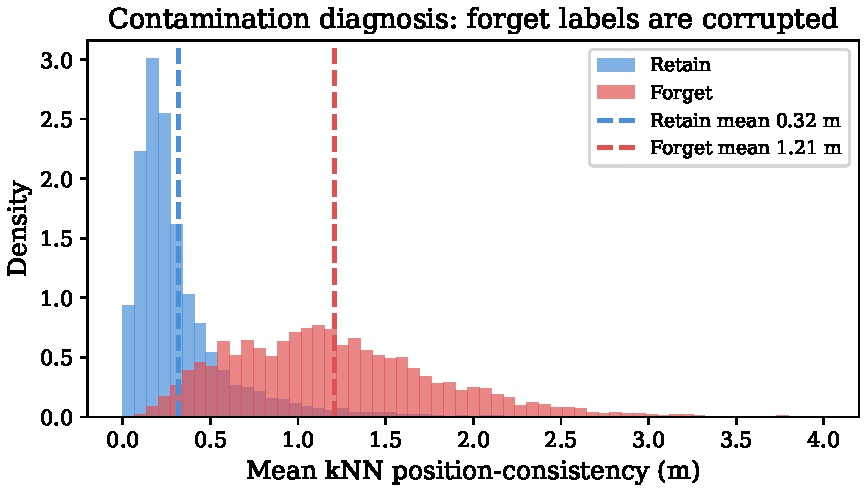
\includegraphics[width=\textwidth]{01_contamination_shift.pdf}
\end{column}
\end{columns}

\end{frame}

% ─────────────────────────────────────────────────────────────────────────────
\section{Two unlearning families}

\begin{frame}{Family A --- Relabel: denoise the labels}

\textbf{Idea}: give the model a \emph{trusted} target for each forget sample, then
fine-tune. The error against the \emph{original} label then equals the corruption.

\medskip
\begin{enumerate}
  \item For each forget sample $i$, find its $k=10$ nearest \textbf{retain} neighbours
    in the 64-dim PCA of $|\mathrm{CSI}|$.
  \item Replace its label with their mean position:
    $\;\ycorr_i = \frac{1}{k}\sum_{j\in\mathrm{kNN}_\Rset(i)} \mathbf{p}_j$
    \quad(retain labels untouched).
  \item Fine-tune on the corrected targets.
\end{enumerate}

\medskip
\begin{block}{Why it works for the metric}
The model learns the true position $\Rightarrow$ for a forget sample the error vs.\ the
\emph{original} (corrupted) label is large and \textbf{transfers exactly} to the test set.
\end{block}

\smallskip
\footnotesize
Result: self-MIA $0.927$, \quad retain error $0.114\,\mathrm{m}$,
\quad forget error $0.861\,\mathrm{m}$.

\end{frame}

% ─────────────────────────────────────────────────────────────────────────────
\begin{frame}{Family B --- Activation-trajectory divergence}

\begin{columns}[T]
\begin{column}{0.52\textwidth}
\textbf{Motivation}: the CNN \emph{already} separates forget from retain internally
(probe AUC \textbf{0.986} at block 5), yet parameter-space dampening (SSD) \emph{fails}
(Fisher importance entangled). \textbf{So act in activation space.}

\smallskip
\textbf{Method} (vs.\ frozen teacher $\fthn$):
\begin{itemize}
  \item \textcolor{cForget}{\textbf{Diverge}} forget pre-ReLU acts off-trajectory.
  \item \textcolor{cRetain}{\textbf{Anchor}} retain post-ReLU acts to the teacher.
  \item $+$ kNN forget-position loss (transferable signal).
\end{itemize}

\smallskip
\footnotesize Real representational change, not just a relabel.
\end{column}
\begin{column}{0.46\textwidth}
\centering
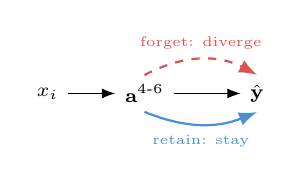
\begin{tikzpicture}[font=\scriptsize, node distance=0.7cm]
  \node (x) {$x_i$};
  \node[right=0.6 of x] (mid) {$\mathbf{a}^{4\text{-}6}$};
  \node[right=0.85 of mid] (out) {$\hat{\mathbf{y}}$};
  \draw[-Latex] (x) -- (mid);
  \draw[-Latex] (mid) -- (out);
  \draw[-Latex,cRetain,thick,bend right=22]
    (mid.south) to node[below,font=\tiny,cRetain]{retain: stay} (out.south);
  \draw[-Latex,cForget,thick,dashed,bend left=28]
    (mid.north) to node[above,font=\tiny,cForget]{forget: diverge} (out.north);
\end{tikzpicture}

\smallskip
  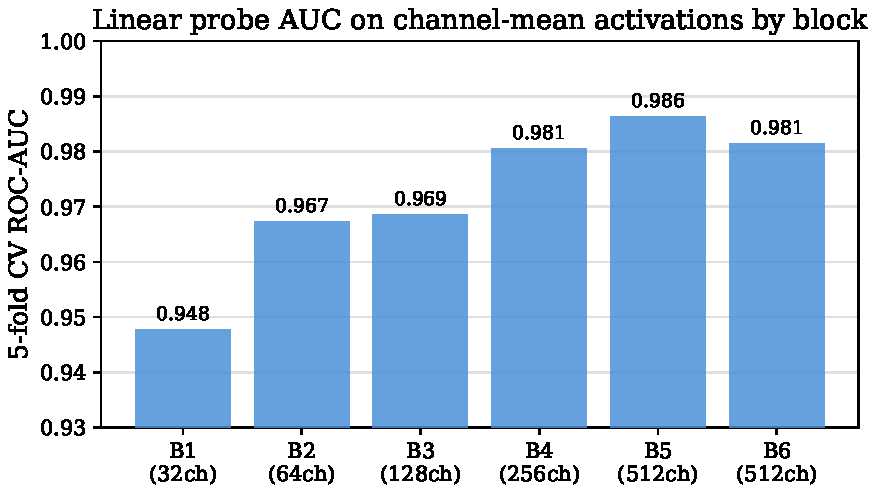
\includegraphics[width=0.8\textwidth]{03_probe_auc_by_block.pdf}
\end{column}
\end{columns}

\end{frame}

% ─────────────────────────────────────────────────────────────────────────────
\begin{frame}{The small ensemble}

\textbf{Why ensemble?} The two families make \emph{complementary} errors:
relabel gives a clean transferable signal; divergence detaches the representation.
Averaging their per-sample errors before the detector yields a \textbf{more separable}
error distribution.

\medskip
\begin{center}
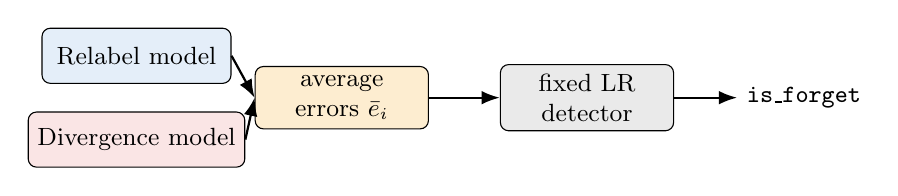
\begin{tikzpicture}[font=\small,
  mod/.style={draw, rounded corners=3pt, minimum width=2.4cm, minimum height=0.7cm, align=center},
  op/.style={draw, rounded corners=3pt, minimum width=2.2cm, minimum height=0.7cm, align=center, fill=cAccent!20},
  arr/.style={-Latex, thick}]
  \node[mod, fill=cRetain!15] (a) {Relabel model};
  \node[mod, fill=cForget!15, below=0.35 of a] (b) {Divergence model};
  \node[op, right=1.5 of $(a)!0.5!(b)$] (avg) {average\\errors $\bar e_i$};
  \node[op, right=0.9 of avg, fill=cTeacher!25] (det) {fixed LR\\detector};
  \node[right=0.8 of det] (out) {\texttt{is\_forget}};
  \draw[arr] (a.east) -- (avg.west);
  \draw[arr] (b.east) -- (avg.west);
  \draw[arr] (avg) -- (det);
  \draw[arr] (det) -- (out);
\end{tikzpicture}
\end{center}

% \medskip
% \begin{itemize}
%   \item Members span both families ($+$ a gradient-ascent variant for diversity).
%   \item Organizers later mandated \emph{single-model} $\Rightarrow$ each family becomes a
%     standalone compliant submission.
% \end{itemize}

\end{frame}

% ─────────────────────────────────────────────────────────────────────────────
\section{Results}

\begin{frame}{Results}

\begin{columns}[T]
\begin{column}{0.52\textwidth}
\footnotesize
\setlength{\tabcolsep}{3pt}
\begin{tabular}{lcccc}
\toprule
Method & self-MIA & retE & fgtE & fgt\% \\
\midrule
Relabel        & \textbf{0.927} & 0.114 & 0.861 & 0.538 \\
Divergence     & 0.881 & 0.139 & 0.769 & 0.519 \\
\midrule
Baseline       & --- & 0.101 & 0.125 & --- \\
\bottomrule
\end{tabular}

\medskip
\scriptsize
retE / fgtE = mean retain / forget error (m).\\
fgt\% = LR test forget rate (true $\approx 0.50$).\\[4pt]
\normalsize
\end{column}
\begin{column}{0.46\textwidth}
  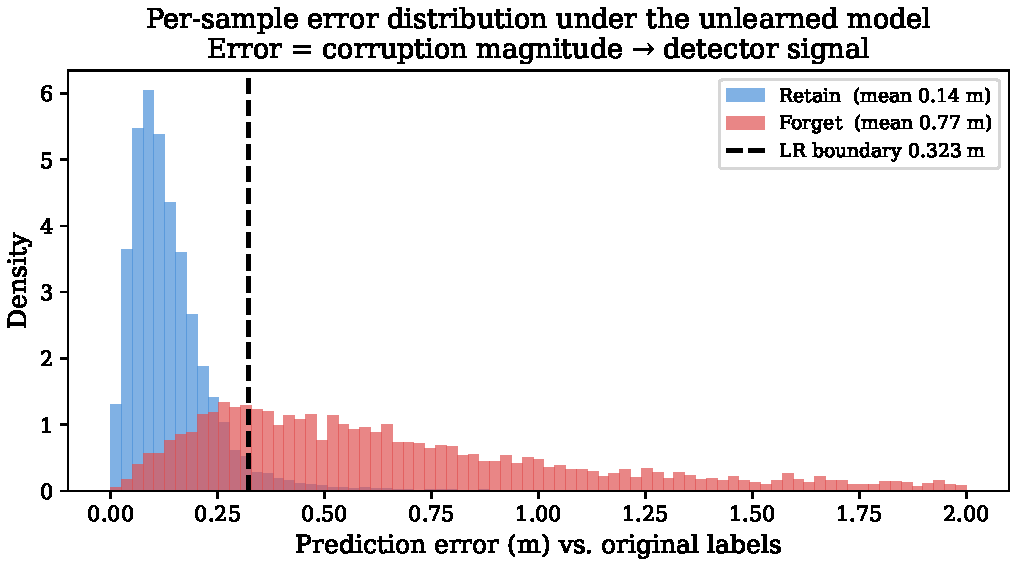
\includegraphics[width=\textwidth]{12_error_distribution.pdf}
\end{column}
\end{columns}

\end{frame}

% ─────────────────────────────────────────────────────────────────────────────
\begin{frame}{Why this is \emph{real} unlearning --- not just relabelling}

\begin{columns}[T]
\begin{column}{0.50\textwidth}
\begin{itemize}
  \item Divergence changes \emph{where} the model maps forget inputs in activation
    space --- direct evidence the internal computation changed.
  \item Forget activations are pushed off the teacher trajectory; retain stays anchored.
  \item \textbf{Ablation}: drop the kNN-position loss and the activation push alone is
    partly train-specific (worse transfer). The two terms are complementary:
    \emph{detachment} $+$ \emph{transferable signal}.
\end{itemize}
\end{column}
\begin{column}{0.48\textwidth}
  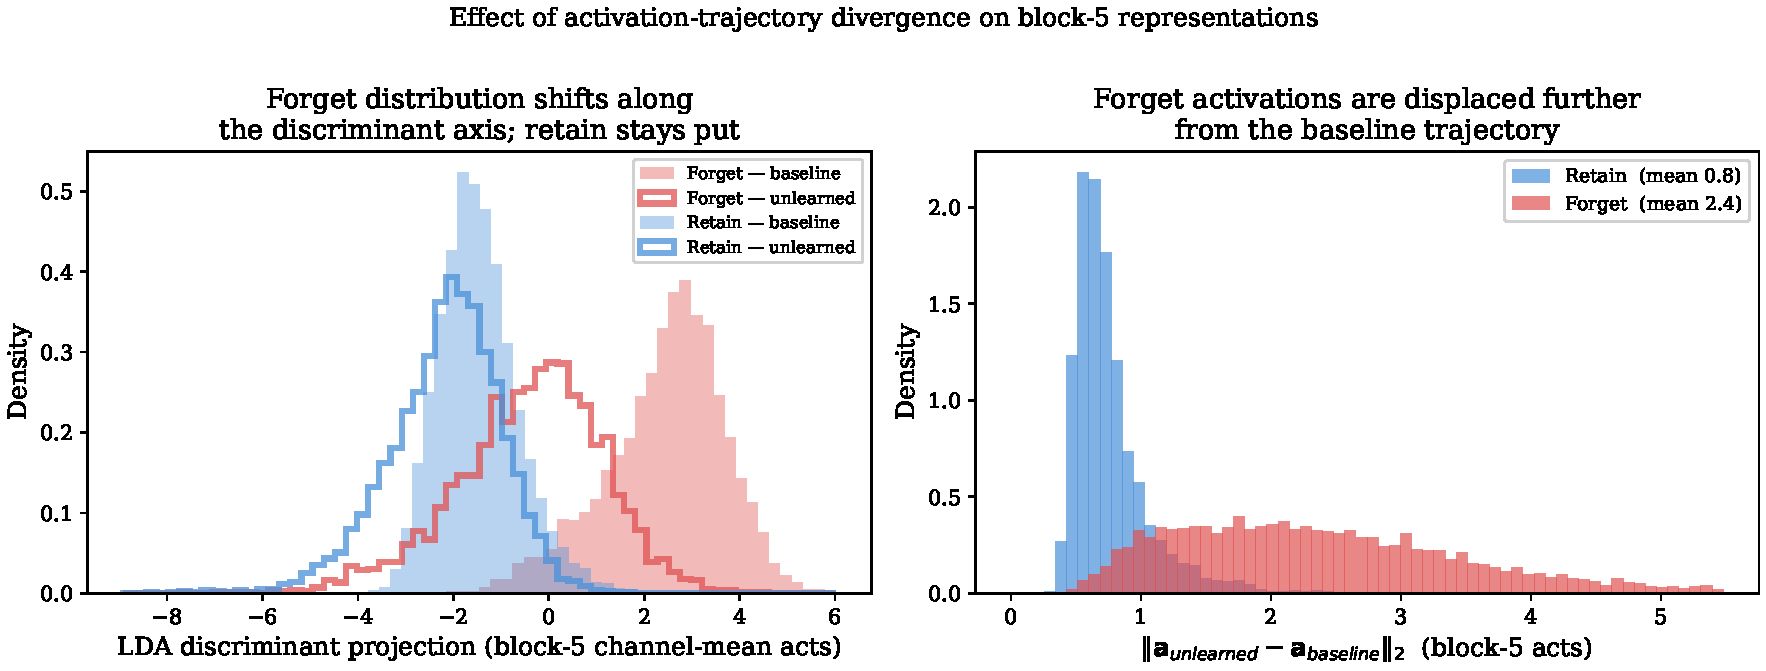
\includegraphics[width=\textwidth]{08_effect_before_after.pdf}

  \scriptsize
  Block-5 activations: \textcolor{cForget}{forget} displaced after unlearning,
  \textcolor{cRetain}{retain} anchored.
\end{column}
\end{columns}

\end{frame}

% ─────────────────────────────────────────────────────────────────────────────
\begin{frame}[fragile]{Conclusion}

\begin{block}{Summary}
\begin{enumerate}
  \item \textbf{Signal}: contamination = corrupted positions; error = corruption magnitude.
  \item \textbf{Family A} relabels with kNN-corrected positions (transferable signal).
  \item \textbf{Family B} diverges forget activations off a frozen teacher (representational).
  \item \textbf{Small ensemble} of both
\end{enumerate}
\end{block}

% \smallskip
% \textbf{One-command repro of a compliant submission}:
% {\scriptsize
% \begin{verbatim}
% python scripts/unlearning/diverge.py \
%     --forget-target knn --beta-anchor 3 --epochs 30
% python scripts/submission/make_submission.py \
%     --ckpt experiments/diverge/model_official_knn_b3.pth \
%     --out my_submission.csv
% \end{verbatim}
% }

% \centering
% \textbf{Thank you!}

\end{frame}

% ─────────────────────────────────────────────────────────────────────────────
% \appendix

% \begin{frame}{Backup: divergence loss \& hyperparameters}

% \footnotesize
% \textbf{Total loss} (student $\fth$, frozen teacher $\fthn$, blocks 4--6):
% \[
%   \mathcal{L} = \Lpos + \beta\,\Lanc + \gamma_t\,\Ldiv + \nu\,\Lnorm + \delta\,\Lposf
% \]
% \begin{itemize}
%   \item $\Lanc$: retain post-ReLU activations pinned to teacher (relative squared dev.).
%   \item $\Ldiv$: hinge-cosine $\mathrm{ReLU}(\cos(\asl,\atl))$ on forget pre-ReLU BN.
%   \item $\Lnorm$: norm-keeper (prevents all-zero collapse). $\Lposf$: kNN forget position.
% \end{itemize}

% \medskip
% \begin{center}
% \begin{tabular}{lll}
% \toprule
% $\beta$ (anchor) & 3.0 & lr $5\times10^{-5}$, Adam, batch 64 \\
% $\gamma$ (diverge) & 0.5 (ramp 2 ep) & 30 epochs, checkpoint ep 24 \\
% $\nu$ (norm) & 0.1 & BN running stats frozen \\
% $\delta$ (kNN pos) & 1.0 & select: max self-MIA, retain $\leq 0.25$\,m \\
% \bottomrule
% \end{tabular}
% \end{center}

% \medskip
% \textbf{$\beta$ calibrates the detector}: tighter anchor $\Rightarrow$ lower train retain
% error $\Rightarrow$ LR threshold shifts $\Rightarrow$ test forget rate $\to 0.50$
% (cross-checked by an unsupervised GMM split --- no leaderboard probing).

% \end{frame}

\end{document}
